\documentclass{article}
\usepackage{wrapfig}
\usepackage{amsmath}
\usepackage{amssymb}
\usepackage{float}
\usepackage{moresize}
\usepackage{graphicx}
\usepackage{amsthm}
\usepackage[dvipsnames]{xcolor}
\usepackage[colorlinks=true, allcolors=black]{hyperref}
\newcommand*{\ClipSep}{0.4cm}
\usepackage{amsfonts}
\usepackage{latexsym}
\usepackage{amssymb}
\usepackage{amsmath}
\usepackage{graphicx} % Required for inserting images
\definecolor{ultramarine}{RGB}{240,120,60}
\definecolor{almond}{rgb}{0.98, 0.81, 0.69}
\usepackage{tikz} 
\definecolor{champagne}{rgb}{0.97, 0.91, 0.81}
\usepackage{geometry}
 \geometry{
 a4paper,
 total={170mm,257mm},
 left=20mm,
 top=20mm,
 }
\title{Do hot streaks exist in sports?}
\author{Hasan Rahman}
\date{ }
\renewcommand*\contentsname{Contents}
\begin{document}
\maketitle
%\begin{document}
\begin{abstract}
Consider a football team that has won its previous three matches. How does this winning streak affect the likelihood of winning the upcoming match? Is there a measurable impact, and how does it influence the team’s chances of victory? In this paper, we aim to examine this relationship and determine whether the results are statistically significant. We will also explore potential explanations for these findings in later sections.
\newline
\end{abstract}
\tableofcontents
\newpage
\section{Introduction and overview}

\subsection{History of the problem} 
\begin{tikzpicture}[remember picture, overlay]
     \node at (11.5,-0.5) {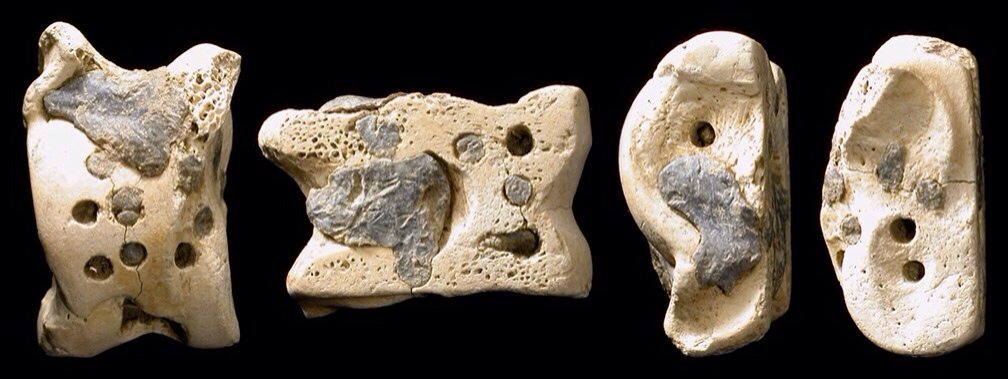
\includegraphics[height=3cm,width=7cm]{Earliest_Dice.jpg}};
     \draw (12.0, -2.25) node {Figure 1: Bone Dice 5-3rd Century BC in Greece\cite{Earliest dice}};
     \node at (3.5,-10.0) {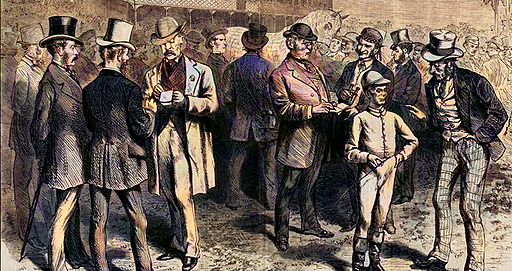
\includegraphics[height=4cm,width=7cm]{Hotpot.png}};
     \draw (3.25, -12.25) node {Figure 2: Horse race betting in the UK\cite{Earliest UK betting}};
\end{tikzpicture}\\[-10pt]
During the Paleolithic period in Mesopotamia, the \newline
earliest six-sided dice date back to about 3000 BC. \newline 
In China, gambling houses were widespread in the \newline
first millennium BC, and betting on fighting \newline
animals was common. Lotto games and dominoes \newline
appeared in China as early as the 10th century.\newline
\newline
Later, it became popular to bet on events, which could cover a myriad of different things, such as horse racing, competitive games, or even the outcomes of gladiator games! It seems that people have been attracted to games of chance since even before written history. While seemingly not very practical, many financial instruments are based on gambling. For example, perhaps the oldest form of gambling involved loaning money, with the interest serving as the reward for taking the risk of lending the capital.\newline
\newline
During the English Civil War, people even bet on who would win the conflict. Would the Cavaliers or the \newline
Roundheads prevail? The modern-day equivalent of this is people betting on platforms like Polymarket for \newline events such as who will be the US president and whether Assad, the leader of Syria, will remain in power by \newline the end of 2024.
\vspace{10mm}

\hspace{67mm}
In England betting would be fairly crude, with most bets being

\hspace{67mm}
even. In other words if you made a bet on if event $X$ happens,

\hspace{67mm}
and you spent $Y$ money. If event $X$ did indeed happen you

\hspace{67mm}
would walk away with $2X$ money.
There is an obvious flaw with

\hspace{67mm}
this system in that it relies on the belief that the probability of

\hspace{67mm}
event $X$ happening is 50$\%$ which is rarely the case.
\\[6\baselineskip]
Therefore, there was a need for bookies to come up with a way to determine the probability of an event occurring so that they could offer appropriate returns. By using past results and data from previous matches, predictive models can be created to calculate the probabilities of various events. These models can go far beyond simply assessing whether team A will win a match; they can also calculate odds for questions such as whether a team will score more than five goals. Using Bayesian statistics, these models can even update odds while the match is in progress. For example, can team A still win despite the fact that it is losing by one point in the first half?
\newline
\newline
Does a team's winning streak meaningfully impact the probability of winning the next match? Answering this question can help develop better models for predictive events, which will enable more accurate odds and, therefore, more competitive rates. For example, better predictive models for car insurance would allow \newline
companies to assess the risk of a customer more easily, enabling them to charge less, as there is less uncertainty associated with the insurance policy.
\newpage
\section{Analysing the data}\label{sec:analyse}
\subsection{Aquiring the data}
To prove or disprove whether hot streaks exist in sports, we need to see if the data supports this hypothesis. We can obtain match results from the Premier League from 1993 to 2023 through Kaggle \cite{Database}. This database contains thousands of games played by teams across the UK, making it ideal for data analysis due to its ample quantity and good quality, as there is no missing data.
\subsection{Proportion of hotstreaks in matches}
\begin{tikzpicture}[remember picture, overlay]
     \node at (7,-4) {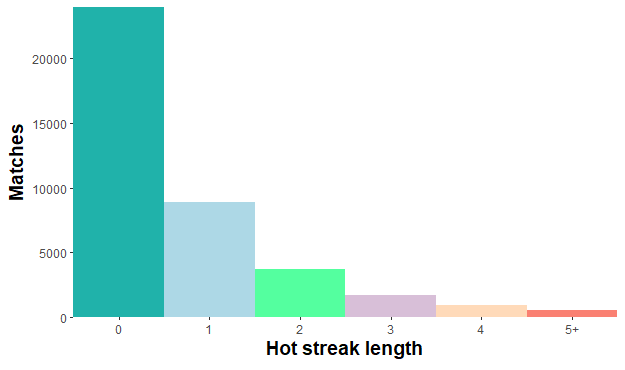
\includegraphics[height=8cm,width=13.5cm]{Rplot.png}};
\end{tikzpicture}
\\[19\baselineskip]
A hot streak can be defined as consecutive wins in matches. From the graph, we find that out of 24,002 games, there are only 8,918 hot streaks of one match, indicating that only 37.2$\%$ of games result in a win for either team. This is due to a large proportion of games ending in a draw. The graph also shows that the longer the hot streak, the more likely it is to continue.
\begin{center}
Hot streak table
\begin{tabular}{lcccccc}
\hline
    &Total&Hot streak of $1$&Hot streak of $2$&Hot streak of $3$&Hot streak of $4$&Hot streak of $5+$\\
\hline
    Matches&$24002$&$8918$&$3657$&$1712$&$882$&$496$\\  
\hline
\end{tabular}
\end{center}
\vspace{8mm}
This table will count a hot streak that ends after matches, as both a hot streak of 1 and a hot streak of 2.
\vspace{8mm}
\begin{center}
End of hot streak table:
\begin{tabular}{lcccccc}
\hline
    Hot streak ends&0&$1$&$2$&$3$&$4$&$5+$\\
\hline
    Matches&$15083$&$5262$&$1945$&$830$&$386$&$496$\\
    Percent of previous&-&$34.9\%$&$37.0\%$&$42.7\%$&$46.5\%$&-\\
\hline
\end{tabular}
\end{center}
From this table, it becomes clearer that the more games a team has won previously, the more likely they are to win again. This provides evidence for the existence of hot streaks.
\newpage
\section{Creating the model}\label{sec:further}
\subsection{Cleaning the data}
First, let’s create a model to predict whether a team will win or lose the next match. To do this, we need to determine the outcomes of each match for each team. The database provides the home and away goals for each match, which can be extracted using an SQL query on BigQuery.\\
\begin{equation*}
  \text{Results for home team}=\begin{cases}
    1, & \text{if home goals$>$away goals}.\\
    0, & \text{otherwise}.
  \end{cases}
\end{equation*}
\begin{equation*}
  \text{Results for away team}=\begin{cases}
    1, & \text{if away goals$>$home goals}.\\
    0, & \text{otherwise}.
  \end{cases}
\end{equation*}
For each team, we can determine whether they won or did not win, which requires different formulas depending on whether they played as the home or away team. We can run another SQL query to find all the matches each team has competed in, whether they were the home or away team, and order the results from oldest to newest. \newline
\newline
Additionally, we will create a field that tracks the result of the previous match for each team. For the first match of each team in this database, this value will be null since it is impossible to determine whether they won or lost their last match. In our model, we can exclude these records, as they lack the previous match result and may introduce noise into the model.
\subsection{Creating a basic model}
To model if a team wins or does not win the next match we can use a generalised linear model. The family will be binomial as match results can only take two values.
\begin{align*}
    &g(Y_i)=\beta_0+\beta_1x_i+\epsilon_i\\
    &Y_i=\text{Probability the team wins the next match}\\
    &\beta_0=\text{Intercept}\\
    &\beta_1=\text{Coefficient of predictor}\\
    &\epsilon_i=\text{Residual}\\
    &x_i=\text{Result from last match} \\
    &g(Y_i)=\text{Link function}
\end{align*}
\subsection{Our results}
Putting our model into R we are able to calculate the parameters which lead to the smallest error in our model.
\begin{center}
Coefficients table:
\begin{tabular}{lcccc}
\hline
    &Estimate&Standard Error&z value&Pr($>|z|$)\\
\hline
    $\beta_0$(Intercept)&$-0.62418$&$0.01712 $&$-36.450$&$<2e-16$\\ 
    $\beta_1$(Coefficient of Predictor)&$0.26324$&$0.0275$&$9.561$&$<2e-16$\\ 
\hline
\end{tabular}
\end{center}
Using the link function we can find what the model predicts.
\begin{align*}
    P(\text{Win match}|\text{Won last match})=41.07\%.\\
    P(\text{Win match}|\text{Lost last match})=34.88\%.
\end{align*}
\newpage

\subsection{Improving the model}
\begin{align*}
    &g(Y_i)=\beta_0+\beta_1x_i+\beta_2x_{i-1}+\beta_3x_{i-2}+\beta_4x_ix_{i-1}+\beta_5x_ix_{i-1}x_{i-2}+\epsilon_i
\end{align*}
To improve our predictive model we can add more data, such as did the team win secound last match it competed in.
\begin{center}
Coefficients table \newline
\begin{tabular}{lcccc}
\hline
    &Estimate&Standard Error&z value&Pr($>|z|$)\\
\hline
    $\beta_0$(Intercept)&$-0.75759$&$0.02406$&$-31.490$&$<2e-16$\\ 
    $\beta_1$(Coefficient of Predictor 1)&$ 0.14053$&$0.03588$&$3.916$&$9e-5$\\ 
    $\beta_2$(Coefficient of Predictor 2)&$0.14893$&$0.03584$&$4.156$&$3.24e-5$\\ 
    $\beta_3$(Coefficient of Predictor 3)&$0.22889$&$0.03057$&$7.487$&$7.07e-14$\\ 
    $\beta_4$(Coefficient of two factor)&$0.17774$&$0.06619$&$2.685$&$0.00725$\\ 
    $\beta_5$(Coefficient of three factor)&$0.12703$&$0.07340$&$1.731$&$0.08351$\\ 
\hline
\end{tabular}
\end{center}
The two and three factor interactions take into account if the team won the previous 2 or 3 matches. From the results of the table, all betas are significant at the level $10\%$, with all betas, except $\beta_5$ being significant at the $1\%$ level.
\begin{align*}
    P(\text{Win match}|\text{Hot streak of 2})=42.79\%.\\
    P(\text{Win match}|\text{Hot streak of 3})=51.64\%.
\end{align*}
\section{Using the model}\label{sec:model}

\subsection{Conclusion}
From the models, we can observe that the relationships are significant and unlikely to have arisen by random chance. Furthermore, there is a notable two-factor interaction related to the outcomes of the previous two matches, significant at the $1\%$ level. This provides strong evidence for the existence of "hot streaks" in sports.\newline
\newline
As for the explanations behind these results, they are likely psychological in nature. Players who have just won a match tend to feel more confident and may thus perform better, increasing their chances of winning the next match. Conversely, the opposite is likely true for players who lost their last match, as decreased confidence may negatively affect their performance.
\newpage
\section{References}


\begin{thebibliography}{11}

\bibitem{Earliest dice}
Traveltoeat.(n.d.). \textit{Ancient Board Games. British Museum.} Retrieved from
\newline
\href{https://traveltoeat.com/ancient-board-games-british-museum/}{https://traveltoeat.com/ancient-board-games-british-museum/}
\bibitem{Earliest UK betting}
Onlinebetting.(n.d.). \textit{The History Of Betting On Football} Retrieved from
\newline
\href{https://www.onlinebetting.org.uk/betting-guides/football/history-of-betting-on-football.html}{https://www.onlinebetting.org.uk/betting-guides/football/history-of-betting-on-football.html}
\bibitem{Database}
Kaggle.(n.d.). \textit{Premier League Matches 1993-2023} Retrieved from
\newline
\href{https://www.kaggle.com/datasets/evangower/premier-league-matches-19922022?resource=download}{https://www.kaggle.com/datasets/evangower/premier-league-matches-19922022?resource=download}
\end{thebibliography}

\end{document}
